\chapter{Visualización computacional. Primeros pasos.}

${ }$\\
\section{Introducción}
${ }$\\

Antes de explicar el algoritmo con el que se obtendrá la imagen de superficies definidas con ecuaciones implícitas empezaré implementando el sistema de rayos, cámara, etc, lo cual servirá de base para después generalizar a superficies mas complejas dadas en sus ecuaciones implícitas. Esta primera implementación incluirá la visualización de superficies en 3D con iluminación sencilla y sin texturas, solo con colores mate. Finalmente para comprobar que esta implementación es correcta se creará una escena con un cubo y una esfera.
${ }$\\

${ }$\\
\section{Rayos, cámara e imagen}
${ }$\\
%%%Explicar Ray-Tracing con alguna imagen

Antes de empezar hay algunas cosas que necesitamos tener antes de empezar a programar la visualización de las superficies. Necesitaremos usar vectores para ello hay definida una clase \textbf{Tupla3f} que venía dada con el código de las practicas de "Informática Gráfica" y que se encarga de almacenar vectores de 3 componentes y realizar las operaciones propias de estos objetos como son el producto escalar, producto vectorial, nomalizado, etc. La forma de almacenar la información de la imagen a visualizar se llevará a cabo mediante una matriz de tantas filas y columnas como filas y columnas de pixeles tenga la ventana donde se va a visualizar la escena. Cada elemento de esta matriz almacenará el color del correspondiente pixel.
	${ }$\\	
	
El color de cada pixel se representará mediante una tupla de tres valores \textbf{double} que se corresponderán los colores rojo, azul y verde (esta representación codificación del color se llama RGB). El valor \textbf{double} que irá de 0.0 a 1.0 indicará la cantidad de ese color.
	${ }$\\	
	
Los rayos y las superficies serán representadas mediante sus expresiones matemáticas. Determinaremos el color de cada pixel mediante el cálculo de la intersección de una recta con la superficie, cada rayo se corresponderá con uno de los pixeles siendo el valor del pixel el color de la superficie del punto donde interseca el rayo (en el caso de que tenga puntos de intersección con la superficie). Para ilustrar como se corresponden los pixeles con los rayos solo basta imaginar una matriz (como un trozo de plano dividido en el espacio), frente a la escena que se quiere visualizar y hacer que de cada elemento de la matriz salga un rayo perpendicular a dicho plano. Esta es una forma de lanzar los rayos aunque la que se usará en este trabajo es diferente.
	${ }$\\	
	
En esta primera parte calcularemos la intersección del rayo con unos objetos mas sencillos de forma directa pues sabemos como calcularla. Pero hay casos en los que por la complejidad de la ecuación esto es mas complicado y necesitamos la ayuda de algoritmos de aproximación de soluciones como son Newton-Raphson y Regula-Falsi que se verán más adelante para encontrar las soluciones de las ecuaciones en forma implícita que definen la superficie.
${ }$\\
	
El color del punto se determina teniendo en cuenta el color de la superficie en dicho punto y, añadiendo la iluminación, también se considerará el ángulo que forma la fuente de iluminación con la normal del objeto en ese punto y el color de la fuente de luz como indica la Ley de Lambert.
	${ }$\\	
%%% Hablar de que están implementados los operadores con tuplas3f, producto escalar etc...

En este caso para visualizar la escena se va a utilizar un simulador de cámara estenopeica. Podemos ver una cámara esteopeica en la Figura \ref{fig:etiq_1}. Este mecanismo de captura de imágenes consiste en una caja cuyo interior es de color negro con un agujero en un lateral y material fotosensible que capturará la imagen en el lateral opuesto.
	${ }$\\	

%%% Imagen Pinhole camera

\begin{figure}[h]
	\begin{center}
		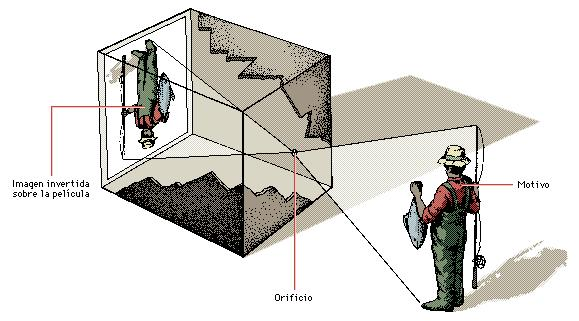
\includegraphics[width=0.6\textwidth]{imagenes/camara-estenopeica.jpg}
	\end{center}
	\caption{Cámara estenopeica. Imagen sacada de Google.}
	\label{fig:etiq_1}
\end{figure}

Primero consideraremos el sistema de referencia de visualización el cual está definido por un punto de origen \textbf{o} y una base ortonormal \{$\textbf{u}$, $\textbf{v}$, $\textbf{w}$\}. Para implementar la cámara, se tomará un rectángulo en el espacio que estará alineado con los ejes $\textbf{u}$ y $\textbf{v}$ como se muestra en la Figura\ref{fig:etiq_3}, este rectángulo se encuentra a distancia $\textbf{s}$ del origen $\textbf{o}$. Llamaremos $\textbf{a}$ y $\textbf{b}$ a las esquinas del rectángulo, que vienen dadas en coordenadas sobre la base \{$\textbf{u}$, $\textbf{v}$, $\textbf{w}$\}.
	${ }$\\

% Imagen propia 1
\begin{figure}[h]
	\begin{center}
		
\includegraphics[width=1.1\textwidth]{imagenes/Imagen1.jpg}
	\end{center}
	\caption{Cálculo de los rayos de visión.}
	\label{fig:etiq_3}
\end{figure}



%%% Hacer yo una imagen con el sistema de coordenadas y el rectangulo dividido con los rayos saliendo del punto.

Sobre este rectángulo tomaremos muestras que se corresponderán con los píxeles que ocupa la ventana de visualización. Volvamos a la Figura\ref{fig:etiq_1} e imaginemos que el rectángulo está dividido en tantas filas y columnas como filas-1 y columnas-1 de pixeles necesitamos para crear la imagen. La forma de tomar el valor para estas muestras se llevará a cabo mediante rayos que pasan por $\textbf{o}$ y por las intersecciones de los segmentos que hemos usado para las divisiones que hemos trazado antes sobre el rectángulo (incluyendo los propios segmentos del rectángulo). Las coordenadas de puntos intersección de segmentos dicha se calculan mediante los siguientes cálculos, estas coordenadas están dadas en la base \{$\textbf{u}$, $\textbf{v}$\}
${ }$\\


\[
	u_i = a_1 + (b_1-a_1) \frac{i}{n_x-1}, \;\;\; 0 \leq i \leq n_x -1,
\]

\[
	v_j = a_2 + (b_2-a_2) \frac{j}{n_y-1}, \;\;\; 0 \leq j \leq n_y -1.
\]
${ }$\\

Entonces los rayos que nos interesan se expresan del siguiente modo en el sistema de referencia de visualización:
${ }$\\

\[
	p_{i,j}(t) = (0,0,0) + t(u_i , v_j, -s).
\]
${ }$\\

En las coordenadas del espacio (estas son las coordenadas en las que está expresada la ecuación de la superficie), esto se traduce en 

\[
	p_{i,j}(t) = e + t( u_i \; u, v_j \; v, -s \; w).
\]

Para poder establecer el punto \textbf{o} de visión y la orientación se calcula el sistema de referencia de visión del siguiente modo:
\begin{itemize}
	\item \textbf{o} : Será el que hemos visto hasta ahora, el punto de visión (donde se encuentra el observador) dado en coordenadas del espacio $xyz$.
	\item \textbf{g} : Se define como un vector en las coordenadas $xyz$ que indica la dirección en la que el observador mira.
	\item \textbf{$v_{up}$} : es un vector que apunta hacia arriba (hacia donde nosotros queramos que sea arriba en la imagen).
	\item \textbf{s} : la distancia de \textbf{o} al rectángulo de visión.
	\item \textbf{a}, \textbf{b} : los que hemos visto con anterioridad, son las esquinas del rectángulo de visión en la base \{$\textbf{u}$, $\textbf{v}$, $\textbf{w}$\}
\end{itemize}
${ }$\\

Con estos datos los vectores de la base ortonormal de visión son
${ }$\\
	\[
		w = - \frac{g}{\parallel g \parallel},
	\]
	\[
		u = \frac{v_{up} \times w}{\parallel v_{up} \times w \parallel},
	\]
	
	\[
		v = w \times u.
	\]
	${ }$\\
	
Si queremos que el rectángulo de visión este centrado con respecto a g hay que asegurarse de que $a_1 = -b_1$ y $a_2 = -b_2$. Además, si no queremos que la imagen resultante se vea estirada en alguno de los ejes \textbf{u} o \textbf{v} debemos asegurarnos de las que divisiones realizadas sobre el rectángulo de visión sean del mismo tamaño tanto para las filas como para las columnas quedando dividido el rectángulo en cuadrados, esto se consigue asegurándose de que
${ }$\\
	\[
		\frac{b_1-a_1}{b_2 - a_2} = \frac{n_x}{n_y}.
	\]
	${ }$\\

En el siguiente código la función $Image$ se encarga de devolver la imagen que se ve desde el punto del observador en una matriz de dimensiones iguales a las del tamaño de la ventana donde se muestra la imagen, la función $interposicionObjeto$ y la Ley de Lambert se verán mas adelante en la parte de iluminación. La función $Inicializar$ se encarga de inicializar los objetos de la escena y otras variables necesarias para la visualización.
${ }$\\

\begin{lstlisting}[style=Consola]
vector<Superficie *> superficies;

double a1, a2, b1, b2;
double s = 6.0;
Tupla3f e = Tupla3f(0,0,8);
Tupla3f g = Tupla3f(0,0,-2);
Tupla3f vup = Tupla3f(0,1,0);
Tupla3f u, v, w;
Tupla3f *image;

LuzDireccional luz = LuzDireccional(Tupla3f(1.5,1.5,1.65), Tupla3f(1, 1, 1));


void Inicializar(int x, int y) {

	superficies.push_back(new Esfera(Tupla3f(0,0,0), 2.0, Tupla3f(0.3, 0.3, 0.3)));
	superficies.push_back(new Cubo(Tupla3f(1.5,1.5,1.5), Tupla3f(2,2,2), Tupla3f(0.5, 0.5, 0.5)));
	superficies.push_back(new Esfera(Tupla3f(-1.5,-1.5,1.5), 0.5, Tupla3f(0.55, 0.55, 0.55)));
	
	image = new Tupla3f [x*y];

	a1=-x/200.0;
	a2=y/200.0;
	b1=-a1;
	b2=-a2;

	w = (-1)*normalized(g);
	u = normalized(vup*w);
	v = w*u;
}

\end{lstlisting}
${ }$\\


\begin{lstlisting}[style=Consola]
Tupla3f* Image(int x, int y){

Tupla3f direccion;

	for(int i = 0; i < x; i++) {
		for (int j = 0; j < y; j++){
			direccion = (a1 + (b1 - a1)*(i/(x-1.0)))*u + (a2 + (b2 - a2)*(j/(y-1.0)))*v -s*w;

			if (!superficies.empty()){

				int indice_min;
				double int_ant;

				primeraInterseccion(direccion, int_ant, indice_min);

				if (int_ant >= 0) {
					image[i*y +j] = luz.LeyLambert( (superficies[indice_min])->getColor(), (superficies[indice_min])->normal(e, direccion, int_ant));

					if (interposicionSuperficie(direccion, int_ant, indice_min) == true) image[i*y +j] = Tupla3f(0, 0, 0);
				}
				else image[i*y +j] = Tupla3f(1, 1, 1);
			}
		}
	}
	return image;
}


\end{lstlisting}
${ }$\\

Cuando hay varios objetos en la escena hay que tener en cuenta cual es el primero que se encuentra el rayo en su recorrido, pues los que encuentre con posterioridad no serán vistos por el observador. Esto es de lo que se encarga la siguiente función, esto es, para cada objeto calcula donde interseca con un rayo dado y devuelve el objeto con el que se encuentra primero y el lugar del rayo donde interseca.
${ }$\\

\begin{lstlisting}[style=Consola]

void primeraInterseccion(Tupla3f direccion, double &min_inter, int &indice_min){

	indice_min = 0;
	min_inter = (superficies[0])->interseccion(*(superficies[0]), e,direccion);

	for (int k = 1; k < (int)superficies.size(); k++) {
		double intersec = (superficies[k])->interseccion(*(superficies[k]), e,direccion);

		if ( (intersec < min_inter && intersec >= 0) || (min_inter == -1 && intersec >= 0) ) {
			indice_min = k;
			min_inter = intersec;
		}
	}
}
\end{lstlisting}
${ }$\\

${ }$\\
\section{Intersección de rayos con objetos}
%$\textbf{4.3. INTERSECCIÓN DE RAYOS CON OBJETOS SENCILLOS}$
${ }$\\

En lo que sigue se van a definir dos clases (Esfera y Cubo) que van a ser subclase de la clase Superficie definida como sigue:

\begin{lstlisting}[style=Consola]
class Superficie {

private :
	Tupla3f color;

public :
	Superficie(Tupla3f col);
	Superficie(const Superficie &sup);
	virtual double interseccion(Superficie &sup, Tupla3f origen, Tupla3f direccion) = 0;
	virtual Tupla3f getColor();
	virtual Tupla3f normal(Tupla3f e, Tupla3f d, double t) = 0;
	virtual double funcion(Tupla3f o, Tupla3f d, double t) = 0;
	virtual double derivada(Tupla3f o, Tupla3f d, double t) = 0;

};

Superficie::Superficie(Tupla3f col){
	color = col;
}

Superficie::Superficie(const Superficie &sup){
	color = sup.color;
}


Tupla3f Superficie::getColor(){
	return color;
}

\end{lstlisting}
${ }$\\

${ }$\\
\subsection{Intersección rayo-esfera}
%$\textbf{4.3.1. Intersección rayo-esfera}$
${ }$\\

Una esfera con centro en $c = (c_x, c_y, c_z)$ y radio $R>0$ se puede representar mediante la siguiente ecuación:
${ }$\\
\[
	(x-c_x)^2 + (y-c_y)^2 + (z-c_z)^2 = 0,
\]
${ }$\\
también se puede expresar como sigue
${ }$\\
\[
	(p-c)\cdot(p-c) - R^2 = 0,
\]
${ }$\\
donde cualquier punto que cumpla la ecuación está en la esfera. En nuestro caso queremos estudiar la intersección de la superficie y un rayo dado por $p(t) = o + td$. Para encontrar los puntos de intersección del rayo con la esfera evaluamos esta expresión en $p(t)$,
${ }$\\
\[
	(o+td-c)\cdot(o+td-c) - R^2 = 0,
\]
${ }$\\
si desarrollamos un poco, obtenemos
${ }$\\
\[
	(d\cdot d)t^2 + 2d\cdot (o-c)t + (o-c)\cdot(o-c) - R^2 = 0,
\]
${ }$\\
podemos observar que esta es una ecuación de la forma $At^2+Bt+C=0$ de la cual podemos conocer sus raíces, que como ya sabemos son
${ }$\\
\[
	t = \frac{-B\pm \sqrt{B^2-4CA}}{2A},
\]
${ }$\\
aplicando esto a nuestro caso, tenemos
${ }$\\
\[
	t = \frac{-d\cdot (o-c) \pm \sqrt{(d\cdot (o-c))^2 - (d\cdot d)((o-c)\cdot(o-c)-R^2)}}{d\cdot d},
\]
${ }$\\
donde como ya hemos visto $t$ indica el lugar del rayo donde alcanza la superficie.
${ }$\\

Para saber si el rayo interseca con la superficie se tendrá en cuenta el signo del discriminante $B^2-4CA$. En el caso de que el discriminante sea igual a cero solo habrá una solución. Si fuese positivo el rayo interseca con la superficie en dos puntos (uno de ellos es el punto a través del cual entra en la superficie y el otra por donde sale de la esfera). Por último, si dicho valor es negativo el valor de la raíz será imaginario y no habrá puntos de intersección de la esfera con el rayo.
${ }$\\
	
A continuación se muestra el código de la clase Esfera la cual permite la creación de una esfera con centro y radio elegidos. Además contiene un método que nos devuelve la distancia del punto origen $\textbf{o}$, de un rayo pasado como parámetro, al punto de intersección mas cercano de la esfera.
${ }$\\

\begin{lstlisting}[style=Consola]
class Esfera : public Superficie {

private :
	Tupla3f centro;
	double radio;

public :
	Esfera(Tupla3f c, double r, Tupla3f col);
	Esfera(const Esfera &sph);
	double interseccion(Tupla3f origen, Tupla3f direccion);
	Tupla3f normal(Tupla3f e, Tupla3f d, double t);

};


Esfera::Esfera(Tupla3f c, double r, Tupla3f col):Superficie(col) {
	centro = c;
	radio = r;
}


Esfera::Esfera(const Esfera &sph): Superficie(sph) {
	centro = sph.centro;
	radio = sph.radio;
}

double Esfera::interseccion(Tupla3f o, Tupla3f d){
	double interseccion = -1;

	double discriminante = (d|(o-centro))*(d|(o-centro)) - (d|d)*(((o-centro)|(o-centro)) - radio*radio);

	if (discriminante > 0) {
		double t0 = ( ( -(d|(o-centro)) + sqrt( discriminante ) ) / ( d|d ) );
		double t1 = ( ( -(d|(o-centro)) - sqrt( discriminante ) ) / ( d|d ) );

		if (t0 > 0) interseccion = t0;
		if (t0 > t1 && t1>0) interseccion = t1;
	}
	return interseccion;
}


Tupla3f Esfera::normal(Tupla3f e, Tupla3f d, double t) {
	return Tupla3f( ((e + t*d)-centro)/radio );
}
\end{lstlisting}
${ }$\\

${ }$\\
\subsection{Intersección rayo-caja}
%$\textbf{4.3.2. Inerseccion rayo-caja}$
${ }$\\

Las cajas de esta sección serán representadas mediante las coordenadas de dos esquinas opuestas $p_0 = (x_0, y_0, z_0)$ y $p_1 = (x_1, y_1, z_1)$ y los lados de dichas cajas estarán alineados con los ejes. Para ver la intersección de los rayos usaremos un método que resulta ser más rápido que comprobar la intersección con cada una de las seis caras y que es la que aparece en el libro \cite{Shirley}.
	${ }$\\	
	
El método al que me refiero considera tres intervalos que se corresponden con cada una de las tres coordenadas, así un punto $(x, y, z)$ que esté dentro del cubo debe cumplir $x \in [x_0, x_1]$, $y \in [y_0, y_1]$ y $z \in [z_0, z_1]$. De este modo, para un rayo dado por $p(t) = o + td$ calcularemos en que intervalo ha de encontrarse $t$ para que el rayo corte la superficie. Para $x \in [x_0, x_1]$,
${ }$\\
\[
	x_0 = o_x + t_{x0}d_x
\]
\[
	x_1 = o_x + t_{x1}d_x
\]
${ }$\\
y despejando $t_{xi}$ en cada ecuación obtenemos que el segmento de rayo que está dentro del cubo se corresponde con
${ }$\\
\[
	t \in [(x_0-o_x)/d_x, (x_1-o_x)/d_x]
\]
${ }$\\

Para definir el intervalo de $t's$ para los que el rayo está en la franja de espacio $[x_0, x_1]$ cuenta si $d_x$ es positivo o negativo, en caso de que sea positivo el intervalo sería el esperado $[t_{x0}, t_{x1}]$, pero en caso de ser negativo sería de la forma $[t_{x1}, t_{x0}]$, por comodidad este intervalo se notará como $[t_{x min}, t_{x max}]$.
	${ }$\\	
% Imagen propia 2
%${ }$\\
\begin{figure}[h]
	\begin{center}
		
\includegraphics[width=0.8\textwidth]{imagenes/Imagen2.jpg}
	\end{center}
	\caption{Cálculo del intervalo de t's para los cuales el rayo está en la superficie.}
	\label{fig:etiq_4}
\end{figure}




El proceso seguido anteriormente para el intervalo en $x$, será el seguido para el intervalo en $y$ y $z$ obteniendo $[t_{y min}, t_{y max}]$ y $[t_{z min}, t_{z max}]$. Una vez calculados los tres intervalos se comprobará si el rayo corta la superficie y cual es el primer punto donde lo hace, esto se hará calculando la intersección de los tres intervalos y comprobando si es vacío o no y en caso de que no sea vacío se devolverá el mínimo del intervalo. Para esto último el algoritmo implementado tomará $t_{min} = max\{t_{x min}, t_{y min}, t_{z min}\}$ y $t_{max} = min\{t_{x max}, t_{y max}, t_{z max}\}$, siendo el intervalo $[t_{min}, t_{max}]$ el intervalo de los $t$ para los que el rayo se encuentra dentro del cubo. Si $t_{min} > t_{max}$ entonces el intervalo es vacío y el rayo no toca al cubo, en caso contrario el algoritmo calcula en qué lugar del rayo se corta por primera vez la superficie, lo que quiere decir que, nos devolverá $t_{min}$. Para ilustrar este método se muestra una simplificación del problema en el espacio 2-dimensional en la Figura\ref{fig:etiq_4}.
${ }$\\	



El código que corresponde a la representación computacional del cubo es el que se muestra a continuación:
${ }$\\

\begin{lstlisting}[style=Consola]
class Cubo : public Superficie {

private :

	Tupla3f esquina1, esquina2;

public :

	Cubo(Tupla3f e1, Tupla3f e2, Tupla3f e3);
	Cubo(const Cubo &squ);
	double interseccion(Tupla3f origen, Tupla3f direccion);
	Tupla3f normal(Tupla3f e, Tupla3f d, double t);

};

Cubo::Cubo(Tupla3f e1, Tupla3f e2, Tupla3f e3):Superficie(e3) {
	esquina1 = e1;
	esquina2 = e2;
}

Cubo::Cubo(const Cubo &squ):Superficie(squ) {
	esquina1 = squ.esquina1;
	esquina2 = squ.esquina2;
}

double Cubo::interseccion(Tupla3f origen, Tupla3f direccion){
	double tx_min, tx_max, ty_min, ty_max, tz_min, tz_max, t0, t1;

	if (direccion.coo[0] > 0) {
		tx_min = (esquina1.coo[0] - origen.coo[0])/direccion.coo[0];
		tx_max = (esquina2.coo[0] - origen.coo[0])/direccion.coo[0];
	}
	else {
		tx_min = (esquina2.coo[0] - origen.coo[0])/direccion.coo[0];
		tx_max = (esquina1.coo[0] - origen.coo[0])/direccion.coo[0];
	}

	if (direccion.coo[1] > 0) {
		ty_min = (esquina1.coo[1] - origen.coo[1])/direccion.coo[1];
		ty_max = (esquina2.coo[1] - origen.coo[1])/direccion.coo[1];
	}
	else {
		ty_min = (esquina2.coo[1] - origen.coo[1])/direccion.coo[1];
		ty_max = (esquina1.coo[1] - origen.coo[1])/direccion.coo[1];
	}

	if (direccion.coo[2] > 0) {
		tz_min = (esquina1.coo[2] - origen.coo[2])/direccion.coo[2];
		tz_max = (esquina2.coo[2] - origen.coo[2])/direccion.coo[2];
	}
	else {
		tz_min = (esquina2.coo[2] - origen.coo[2])/direccion.coo[2];
		tz_max = (esquina1.coo[2] - origen.coo[2])/direccion.coo[2];
	}

	if (tx_min > ty_min) t0 = tx_min;
	else t0 = ty_min;
	if (tz_min > t0) t0 = tz_min;

	if (tx_max < ty_max) t1 = tx_max;
	else t1 = ty_max;
	if (tz_max < t1) t1 = tz_max;


	if (t0 < t1) return t0;
	else return -1;
}


Tupla3f Cubo::normal(Tupla3f e, Tupla3f d, double t) {
	if ( abs((e+t*d).coo[0] - esquina2.coo[0]) <= 0.01 ) return Tupla3f(1,0,0);
	else if ( abs((e+t*d).coo[1] - esquina2.coo[1]) <= 0.01 ) return Tupla3f(0,1,0);
	else if ( abs((e+t*d).coo[2] - esquina2.coo[2]) <= 0.01 ) return Tupla3f(0,0,1);
	else if ( abs((e+t*d).coo[0] - esquina1.coo[0]) <= 0.01 ) return Tupla3f(-1,0,0);
	else if ( abs((e+t*d).coo[1] - esquina1.coo[1]) <= 0.01 ) return Tupla3f(0,-1,0);
	else if ( abs((e+t*d).coo[2] - esquina1.coo[2]) <= 0.01 ) return Tupla3f(0,0,-1);
}
\end{lstlisting}
${ }$\\

${ }$\\
\section{Iluminación}
%$\textbf{4.4. ILUMINACIÓN}$
${ }$\\

La iluminación hace las imágenes más realistas y nos permite apreciar la profundidad de los objetos. En esta sección veremos una implementación de la iluminación sencilla que solo dependerá de la normal de la superficie y la dirección de incidencia de la fuente de iluminación. 
${ }$\\

Como se muestra en la Figura\ref{fig:etiq_5}, el rayo de visión interseca la superficie en un punto iluminado, este rayo esta definido por el vector \textbf{d} y a partir de él definimos el vector unidad \textbf{e} el cual tiene la misma dirección de \textbf{d} pero sentido opuesto:
${ }$\\

%%% Hacer una imagen como la del libro pero que sea propia

\[
	\textbf{e} = - \frac{\textbf{d}}{\|\textbf{d}\|},
\]
${ }$\\
este vector será prescindible a la hora de añadir la iluminación, se utiliza para materiales que cambian su brillo de posición cuando el observador cambia también la suya.
${ }$\\


El vector \textbf{l} indica la dirección desde la que llega la luz y \textbf{n} el vector normal a la superficie. Con todo esto la Ley de Lambert sería
${ }$\\
\[
	L = ER(\textbf{n}\cdot \textbf{l}),
\]
${ }$\\
esta ley nos da el valor del color del pixel habiendo añadido la iluminación. En esta fórmula $E$ es el valor del color de la fuente de luz y $R$ el color del punto de incidencia, el producto de ellos es componente a componente. Debemos observar que $L$ puede ser negativo, cuando esto ocurre podemos tomar dos caminos, uno de los cuales es hacer cero los valores negativos, este es el que se va a usar aquí es el que vamos a usar, y otro consiste en tomar el valor absoluto.
	${ }$\\	


%Imagen propia 3
\begin{figure}[h]
	\begin{center}
		
\includegraphics[width=0.7\textwidth]{imagenes/Imagen3.jpg}
	\end{center}
	\caption{Elementos geométricos para la implementación de la luz.}
	\label{fig:etiq_5}
\end{figure}





Hasta ahora solo se ha visto como implementar sombras con un solo objeto pero cuando hay más objetos en la escena hay sombras que se producen cuando un objeto se interpone entre la fuente de luz y otro objeto.
	${ }$\\	
	
En este caso tomamos un rayo que sale de un punto \textbf{q}, del que se quiere calcular su color, en dirección \textbf{l} pero sentido opuesto. Si el rayo interseca con otra superficie el valor de $L$ se pone a cero en caso contrario se calcula el valor del color mediante la Ley de Lambert. Esto se ilustra en la Figura\ref{fig:etiq_6}. No se tendrán en cuenta objetos que intersequen en un valor de t negativo o cero.
	${ }$\\	
	
También puede ocurrir que por razones de precisión finita haya puntos que se oscurezcan por que se haya calculado que el rayo de sombra interseca a la propia superficie (la que contiene a q), para evitar este problema lo que hacemos es considerar solo las intersecciones que tienen un $t > \epsilon$ para $\epsilon > 0 $.
	${ }$\\	

\begin{figure}[h]
	\begin{center}
		
\includegraphics[width=0.8\textwidth]{imagenes/Imagen4.jpg}
	\end{center}
	\caption{Implementación de sombras para mas de un objeto. El punto en rojo se coresponde con un punto al que no le da la luz por que la intercepta otro objeto. En cambio el punto en azul es alcanzado por la luz ya que no hay objetos que se la tapen.}
	\label{fig:etiq_6}
\end{figure}

El siguiente código implementa la fuente de luz que solo tiene como atributos la dirección con la que la luz incide en los objetos y el color de la misma. El código que implementa la iluminación se ha mostrado con anterioridad en la función $Image$. A continuación se muestra el código de la función $interposicionObjeto$ el cual es llamado desde la función $Image$ que ya se ha visto anteriormente. Está función se encarga, para cada rayo, de comprobar si (para cada punto visible para el observador) hay una superficie que se interpone entre la luz y dicho punto del objeto para hacer que ese punto se vea sombreado. Devuelte true si hay una superficie que se interpone o falso en caso contrario.
	${ }$\\



\begin{lstlisting}[style=Consola]
class Iluminacion{

private:

	Tupla3f color;

public:

	Iluminacion(Tupla3f col);
	virtual Tupla3f LeyLambert(Tupla3f objColor, Tupla3f normal, Tupla3f punto);
	virtual Tupla3f getDireccion(Tupla3f punto)=0;
};

Iluminacion::Iluminacion(Tupla3f col){

	color = col;
}

Tupla3f Iluminacion::LeyLambert(Tupla3f objColor, Tupla3f normal, Tupla3f punto) {

	Tupla3f L = Tupla3f(color.coo[0]*objColor.coo[0], color.coo[1]*objColor.coo[1], color.coo[2]*objColor.coo[2]) * (normal | getDireccion(punto));

	return L;
}
\end{lstlisting}
${ }$\\


\begin{lstlisting}[style=Consola]

class LuzDireccional : public Iluminacion {

private:

	Tupla3f direccion;

public:

	LuzDireccional(Tupla3f d, Tupla3f c);
	Tupla3f getDireccion(Tupla3f punto);
};

LuzDireccional::LuzDireccional(Tupla3f d, Tupla3f c):Iluminacion(c) {

	direccion = d;
}

Tupla3f LuzDireccional::getDireccion(Tupla3f punto) {

	return direccion;
}


\end{lstlisting}
${ }$\\

\begin{lstlisting}[style=Consola]

bool interposicionSuperficie(Rayo rayo, double min_inter, int indice_min){

	bool inter = false;
	int k=0;

	while ( (k < (int)superficies.size()) && !inter) {

		if ( ((superficies[k])->interseccion(*(superficies[k]),  Rayo(rayo.puntoRayo(min_inter), fuentesLuz[0]->getDireccion(rayo.puntoRayo(min_inter))) ) >= 0.0) && (k!= indice_min) )  inter = true;
		k++;
	}
	
	return inter;
}
\end{lstlisting}
	${ }$\\
	
Adicionalmente, la clase luz puntual, la cual almacena el punto donde está la fuente de luz y desde la que salen los rayos de luz en todas direcciones.

\begin{lstlisting}[style=Consola]
class LuzPuntual : public Iluminacion {

private:

	Tupla3f posicion;
	Tupla3f color;

public:

	LuzPuntual(Tupla3f p, Tupla3f c);
	Tupla3f getDireccion(Tupla3f punto);
};

LuzPuntual::LuzPuntual(Tupla3f p, Tupla3f c):Iluminacion(c) {

	posicion = p;
	color = c;
}

Tupla3f LuzPuntual::getDireccion(Tupla3f punto) {

	return normalized(posicion - punto);
}
\end{lstlisting}
${ }$\\


Finalmente para comprobar que lo que hemos programado hasta ahora funciona correctamente he realizado una prueba usando los objetos que creé y almacené en el vector $superficies$ que se ve en el código presentado al principio en la función $Inicializar$. Después de ejecutarlo el resultado fue el que se muestra en la Figura \ref{fig:etiq_9}.
${ }$\\

\begin{figure}[h]
	\begin{center}
		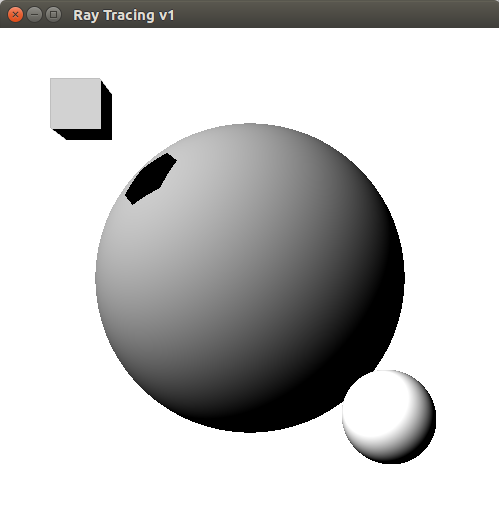
\includegraphics[width=0.8\textwidth]{imagenes/prueba.png}
	\end{center}
	\caption{Ejemplo de comprobación}
	\label{fig:etiq_9}
\end{figure}

